\documentclass[11pt]{article}
\usepackage{geometry}                
\geometry{letterpaper}                   

\usepackage{graphicx}
\usepackage{epstopdf}
\usepackage{amssymb}
\usepackage{epstopdf}
\usepackage{natbib}
\usepackage{amssymb, amsmath}
\usepackage{booktabs}
\usepackage{multicol}
\usepackage{color}           
\usepackage{hyphenat}
\usepackage{booktabs}
\usepackage{hyperref}



\DeclareGraphicsRule{.tif}{png}{.png}{`convert #1 `dirname #1`/`basename #1 .tif`.png}
\parindent 0cm

%\title{Title}
%\author{Name 1, Name 2}
%\date{date} 

\begin{document}



\thispagestyle{empty}

\begin{center}

\includegraphics[width=5cm]{ETHlogo.eps}

\bigskip


\bigskip


\bigskip


\LARGE{ 	Lecture with Computer Exercises:\\ }
\LARGE{ Modelling and Simulating Social Systems with MATLAB\\}

\bigskip

\bigskip

\small{Project Report}\\

\bigskip

\bigskip

\bigskip

\bigskip


\begin{tabular}{|c|}
\hline
\\
\textbf{\LARGE{Insert Title Here}}\\
\textbf{\LARGE{...}}\\
\\
\hline
\end{tabular}
\bigskip

\bigskip

\bigskip

\LARGE{Name 1 \& Name 2}



\bigskip

\bigskip

\bigskip

\bigskip

\bigskip

\bigskip

\bigskip

\bigskip

Zurich\\
May 2008\\

\end{center}



\newpage

%%%%%%%%%%%%%%%%%%%%%%%%%%%%%%%%%%%%%%%%%%%%%%%%%

\newpage
\section*{Agreement for free-download}
\bigskip


\bigskip


\large We hereby agree to make our source code for this project freely available for download from the web pages of the SOMS chair. Furthermore, we assure that all source code is written by ourselves and is not violating any copyright restrictions.

\begin{center}

\bigskip


\bigskip





\begin{tabular}{@{}p{3.3cm}@{}p{6cm}@{}@{}p{6cm}@{}}

\begin{minipage}{6cm}
\vspace{2mm} 
\large Tim Weber
\vspace{\baselineskip}
\end{minipage}


\begin{minipage}{6cm}
\vspace{2mm} 
\large Jan Speckien
\vspace{\baselineskip}
\end{minipage}

\begin{minipage}{6cm}
\vspace{2mm} 
\large Patrice Gobat
\vspace{\baselineskip}
\end{minipage}

\begin{minipage}{6cm}
\vspace{2mm} 
\large Lionel Gulich
\vspace{\baselineskip}
\end{minipage}


\end{tabular}


\end{center}
\newpage

%%%%%%%%%%%%%%%%%%%%%%%%%%%%%%%%%%%%%%%



% IMPORTANT
% you MUST include the ETH declaration of originality here; it is available for download on the course website or at http://www.ethz.ch/faculty/exams/plagiarism/index_EN; it can be printed as pdf and should be filled out in handwriting


%%%%%%%%%% Table of content %%%%%%%%%%%%%%%%%

\tableofcontents

\newpage

%%%%%%%%%%%%%%%%%%%%%%%%%%%%%%%%%%%%%%%



\section{Abstract}
%abstract:
% numbers to detailed
%problem
%what was done before
%why old has failed
%what is left open
% how we address it = intro
%sentnce for each main result
%close it 


% no matlab writing
% explore amount of risktaking
% numbers replace with intermediate
% numbers not clear what they mean
%elaborated strategy not 
%finish with general outcome of this study


%how to deal with errors, talk about them

%section talking about robustness, why parameters are logical
%sigma validation aside

In the recent years Texas Hold’em has been increasingly popular amongst all age groups. Therefore, the aim of this study was to research how different strategies perform against each other in a heads-up.\\ Hence we wrote a program that simulates a game of Texas Hold’em in which all feasible strategies compete against each other. In our model the strategy is represented by a single variable called risk factor that holds the willingness of taking risks.\\ In the model the strategy was constant over the course of a game. For the latter part one player could adjust his risk factor based on different learning algorithms, which then are compared with each other.\\ The results showed, that a very passive strategy always lost. This corresponds to the outcome of a real heads up, where the passive player has a disadvantage due to the blinds. For two players in general the less extreme strategy showed to be more effective. However, this characteristic could not be verified to match reality. Concerning the learning algorithms, a significant increase in the average number of games won by the learning player could be observed.\\
This indicates that with an adaptive strategy an important increase in the average games won can be achieved, also in real Texas Hold’em.\\ The simple model proved to be well suited to quickly observe changes in single variables like the blind value. It can also be easily expanded to observe other variables. Nevertheless, a comparison with actual game data is needed to verify the model.


\section{Individual contributions}

The commonly used models for Texas Hold'em are mostly based on stochastical probability, which makes the implementation of algorithms highly complicated. Thus we decided to write our own simulation in order to simplify the problem using as few variables as possible. All further results and conclusions are based on our program.


\section{Introduction and Motivations}

Texas Hold’em is a variation of the card game Poker and is throughout casinos, tournaments and private people amongst the most popular of its kind. The goal of the game consists in winning all the money, or from here on called “chips” (virtual currency), from the other players at the table. As soon as someone has no more chips left, he lost and has to leave the table.
Every round consists of different stages of card dealing and then successive betting. In each stage a player can decide if and how much chips he wants to play according to some rules and by evaluating their private cards called “hand” and the cards open on the table named sequentially “flop”, “turn” and “river”.
The total amount of chips from all the players in one round is called “pot”. Every round ends with either one player getting the whole pot or sometimes with a split of the pot, if two or more players have an equivalent “score” in the end of the round. The score is the highest possible combination of the private and public cards available according to a fixed ranking.
\\
The game can be played with a varying number of people and for simplicity be subdivided into two parts: “Group stage” and “Heads up”, whereby the main difference lies in the number of people playing. In a heads up the last two remaining players are gambling for the overall victory and therefore every game of Texas Hold’em will end with a heads up.
\\
Every player has his own strategy, where some players like to play more conservative by not betting often and waiting for better cards and others play more aggressive by betting more often and trying to bluff his opponent. An important aspect of the game is the “blinds”, since they force the players to bet a fixed amount before the first cards are dealt. The blinds move forward by one player after every round. They guarantee that no player only can wait for the perfect cards and that there are always chips in the pot that can be won.
\\							
We all agree that Texas Hold’em is about knowing your opponent and play “smarter” or “better” than him. Therefore it is not possible to have a fixed strategy. One has to be able to adjust his strategy depending on the way the opponent is playing and vice-versa.\\
 
Hence we all often wondered what would be good strategies to best adjust to one’s opponent and in particularly how effective such strategies are. To make a valuable assumption about the effectiveness of such a strategy, one would need to play an enormous amount of games to formulate a statistically speaking valid statement. If a whole game or at least some parts of it can be simulated repeatedly under different circumstances and with varying strategies, then one could gain deeper insights into Texas Hold’em and possibly develop an applicable strategy or at least compare different approaches.


\section{Model and implementation}

This section serves to understand how we implemented the simulation. Expressions are introduced that we use throughout the report. One can find the whole program on GitHub \footnote{https://github.com/atlas000/project-poker-msssm} in the folder code. 

\subsection{main.m}

The script ultra-main plays all the different risk factors against each other and saves the amount of wins by player1 in a matrix.\\

The risk factor determines the character of a player. It is stored with a number between 0 and 1, whereas a smaller number represents a riskier player that plays a hand even if his score is not that high and vice versa.

%is that during the game a player has to decide whether to call or to drop out of a hand. In other words, he has to evaluate if his score is good enough to continue playing.

The function main.m serves as an interface where one can decide on the settings through variables which then get passed on to the function game.

 

\subsection{game.m}

The function game.m is used to call the functions headsup/2. Like in real poker game.m continues to deal new hands until one player has run out of money. It is alternately calling two functions that differ only in which player has to pay the blind.\\

As described above, a blind is essential to the game of Texas Hold'em. A player has to pay some money into the pot without having seen his cards yet. That way if a player is very passive, he looses money anyway and has to become more active at some point. \\

In our model only a single fixed blind has been implemented, since in a heads up only the difference in blinds is relevant.

 

\subsection{headsup.m}

The headsup.m function simulates one hand which consists of up to four rounds. With every new card unveiled each player faces the decision whether to place a bet or not. Their action is determined by comparing their risk factors to their score. In total this scenario occurs up to four times per hand. If both players want to play until the end, a showdown determines the winner. Meaning that they have to show their cards and the one with the better score wins the hand and receives the pot.\\

In the first round, the "preflop", one player has to pay the blind and each player gets a set of playing card.\\

The main aspect making poker a complicated game to simulate is its use of cards. Hence our main goal was to find a model, which did not require the implementation of a deck of cards. In order to achieve a similar effect every player is given a random number, called "card value". The number reaches from 0 to 1 and represents the quality of the hand, whereas 0 would be the worst hand and 1 the best.\\

In the next three rounds the "flop", "turn" and "river" new cards get unveiled on the table. So the score of the players' hands has to be adjusted.

 

\subsection{adujstCardValue.m}

At the heart of this simulation lies the adjustCardValue function, which recalculates the card value of a player.\\

Important criteria are that the cards correlate with each other, so if a player has good cards it is likely that his hand is still good when a new round is played. Also it should be possible for a value to reach the whole spectrum of card quality from 0 to 1. This is important because if one has a bad starting hand it should still be possible, with some luck, to get the best hand possible after the flop. Hence every value should be possible to receive but not with the same probability.\\


\subsection{Learning models}
An important part of real Texas Hold’em is to obtain an advantage by estimating the strategy of your opponent and to react accordingly.
In this model two different approaches for learning algorithms have been chosen to optimise a player's strategy, under the assumption that the opponent keeps his risk factor constant.
\begin{itemize}
\item One approach is minimise the losses and thus maximise the profit of a player. This model analyses a player's own performance.
% and therefore only depends on his strategy 
\item  The other approach was to first analyse the play of the opponent and then choose the optimal strategy to best counter the other player. This of course is only possible if all outcomes for all strategies are known.\\
\end{itemize}

\subsubsection{Iteration model}
This learning algorithm analyses the loss of the last hand, because if the last hand has been won there is no need to adapt the strategy. So after every hand one of the following scenarios takes place:\\

\renewcommand{\arraystretch}{1.4}
\begin{tabular}{ p{6.45cm}  p{5.1cm}  p{2.4cm}}
%\hline
Validation & Interpretation & Action\\
%\end{tabular}
\addlinespace
%\begin{tabular}{ p{6.2cm}  | p{5.1cm} | p{2.7cm}}
\hline
\hline

Capital($t+1$) $>=$ Capital($t$) &	The player had equal or better cards, or the hand has not been played&
risk factor $r$ will not be changed \\
%\hline
\addlinespace
Capital$(t+1) ==$ Calpital$(t)-4$	&	The player has lost after the showdown and is thus to agressive & \ r=r+0.012\\
%\hline
\addlinespace
Else (Capital dropped by 1,2 or 3) &	The player is to passive, since it did not come to a showdown & \ r=r+0.003\\
%\hline
\end{tabular}




\subsubsection{Count and gauge model}

The main goal behind analysing the opponent’s way of playing is to correctly estimate his risk factor, in order to adapt one’s risk factor afterwards. 
This algorithm is accomplished in two consecutive steps:
 
Firstly it keeps track of the number of times the opponent decides to play the initial round when he is not forced to do so by the blind. The ratio between this value and the total amount of rounds played can then be used as a measurement to estimate the opponent’s risk factor:
 $$
\textnormal{risk factor} \approx 1 - \dfrac{\textnormal{\# rounds}}{\textnormal{\# rounds played}}
 $$
The second part consists of finding the optimal counterpart to the estimated risk factor. For that reason we evaluated results obtained by previous simulations. The data obtained indicates that for every risk factor chosen, there is at least one optimal counterpart. After extracting these values the algorithm adjusts the own risk factor.

 

\subsubsection{Threshold model}

The target of this learning model is to determine the risk factor from the opponent, which then enables to find the optimal risk factor for the learning player.
Everytime a showdown is conducted the learning player gets to know the score from his opponent . Because the opponent has continued the hand with this score until the showdown, it is known, that the risk factor from the opponent has to be lower than said score. With every showdown executed the possible values for risk factor of the opponent can be narrowed down, leaving a threshold which has to be undershot by the opponent's risk factor.


The optimal risk factor for the learning player can then be determined with the data obtained by previous simulations. This data includes the win probality of both players for all possible combinations of risk factors between both players. Determining the optimal risk factor then only is a matter of finding the maximum for a given opponent strategy.



%\section{Description of the Model}
%
%\subsection{Generic Model}
%
%\paragraph{Card replacement}
%The main aspect making poker a complicated game to simulate is its use of cards. Hence our main goal was to find a model, which did not require the implementation of a deck of cards. In order to achieve a simular effect every player is given a random number, called "card value" between zero and one, representing the quality of his hand, whereas 0 would be the worst hand and 1 the best. 
%
%\paragraph{Card value adjustment}
%In poker, new cards countinuously are being unveiled, which changes the score of a hand. This aspect has to be taken in account by modifying the card value during the one hand. The impact of the new cards on the score of a hand decreases during the game. We implemented this such as in the beginning the new card value varies a lot and at the end it is more likely to stay around the old card value.
%
%\paragraph{Risk factor}
%During the game a player has to decide whether to call or to drop out of the heads up, meaning he has to evaluate if his score is good enough to continue playing. This is achieved with the so called "risk factor", which determines the character of a player. It is again a number between 0 and 1, whereas a smaller number represents a riskier player.
%
%\paragraph{Blind}
%Just as in real Poker a blind has been implemented. At the beginning of every heads up, alternately one player has to pay the blind without having seen his cards yet. In our model only a single fixed blind has been implemented, since in a heads up only the difference in  blinds is relevant.
%
%\paragraph{Betting}
%With every new card unveiled alternately the players face the decision whether to place a bet or not. Their action is determined by comparing their risk factors to their score. In total this scenario occures up to four times per hand. Each time both players can place a bet of one chip.
%
%\paragraph{Showdown}
%A showdown occurs when both players bet until the end. There the winner of a hand is evaluated and he receives all chips bet (pot). If both players have the same score the pot is split.
%
%
%\subsection{Learning models}
%An important part of real Texas Hold’em is to obtain an advantage by estimating the strategy of your opponent and to react accordingly.
%However in this model two different approaches for learning algorithms have been chosen to optimize a players strategy:
%\begin{itemize}
%\item One approach was to adapt the strategy in order to minimize the losses and thus maximize the profit of a player. This model analyses a players own performance. (model Tim \& Jan)% and therefore only depends on his strategy 
%\item  The other approach was to first analyse the play of the opponent and then choose the optimal strategy to best counter the other player, this of course is only possible if all outcomes for all strategies are known to the player which was the case in this model (model Patrice \& Lionel)\\
%\end{itemize}
%Furthermore we took the assumption, that the opponent plays strictly regular and thus no ability to learn.
%
%\subsubsection{Threshold model}
%
%The target of this learning model is to determine the risk factor from player 2, which then enables to find the optimal risk factor for player 1 for which his winning probability is increased.
%Everytime a showdown is conducted player 1 gets to know the cardvalue from player 2. Because player 2 has continued the headsup with this cardvalue until the showdown it is known, that the risk factor from player 2 has to be lower than said cardvalue. With every showdon executed the possible values for risk factor from player 2 can be narrowed down, leaving a threshold which has to be undershot by player 2's risk factor.
%
%
%The optimal risk factor from player 1 can then be determined with the "50 Games" Matrix. This matrix includes the winprobality for player 1 for all possible combinations of risk factors between both players. Determining the optimal risk factor for player 1 is then only a matter of finding the maximum in a certain area of the matrix.
%
%
%
%
%\subsubsection{iteration model}
%This learning algoritm analyzes the loss of the last hand, because if the last hand has been won there is no need to adapt the strategy. So after every hand one of the following scenarios take place\\
%\renewcommand{\arraystretch}{1.4}
%\begin{tabular}{ p{6.45cm}   p{5.1cm}  p{2.4cm}}
%%\hline
%Validation & Interpretation & Action\\
%%\end{tabular}
%\addlinespace
%%\begin{tabular}{ p{6.2cm}  | p{5.1cm} | p{2.7cm}}
%%\hline
%CapitalP-($t+1$) $>=$ Capital($t$) &	The player had equal or better cards, or the hand has not been played&
%r will not be changed \\
%%\hline
%\addlinespace
%CapitalP-$(t+1) ==$ Calpital$(t)-4$	&	The player has lost after the showdown and is thus to agressive & \ r=r+0.012\\
%%\hline
%\addlinespace
%Else (CapitalP- dropped by 1,2 or 3) &	The player is to passive, since it did not come to a showdown & \ R2=R2+0.003\\
%%\hline
%
%
%\end{tabular}
%
%\subsubsection{Count and gauge model}
%
%The main goal behind analysing the opponent’s way of playing is to correctly estimate his risk factor, in order to adapt one’s risk factor afterward. 
%Our algorithm accomplishes this in 2 consecutive steps:
% 
%(Only necessary in case it is not mentioned In the introduction The opponent plays strictly regular, and every card value is equally alike.) Hence the algorithm keeps track of the number of times the opponent decides to play the first round when he is not forced to do so by the blind, called “nroundsplayed”. The ratio between this value and the total amount of rounds played called “nrounds” can then be used as a measurement to estimate the opponent’s risk factor, called “RF” as followed:
% 
%Formula RF= 1 –(nrounds/nroundsplayed)
% 
%The second part consist of finding the optimal counterpart to the risk factor estimated in above. For that reason we evaluated results obtained by simulating almost all possible combination of strategies. The data obtained indicates, that for every risk factor chosen, there is at least one optimal counterpart. After extracting these values, the algorithm can adjust the own risk factor referring to these values.
% 
%Advantages:
%·         With an increasing number of rounds, the estimation continuously gets better
%·          On a long run he will always play the most suitable strategy and optimize his return.
%·         It reaches a good estimation of the opponents risk factor already after a few rounds
%·         The algorythm could also use the rounds where the other player has to pay the blind by counting the number of consecutive rounds he plays and applying the same strategy just by including the models standartdeviation into the calculus. This would lead to a faster estimation of the opponents risk factor.
% 
%Disadvantag es:
%·         The algorithm requires a precise knowledge of all possible outcomes and therefore is only applicable in the same circumstances the data was obtained.
%We had to take in account an estimation error as long as the number of hands played is low.
%
%l
%
%
%
%
%
%
%\section{Implementation}
%In this chapter the Implementaion of the simulation is discribed in the following manner:
%\begin{itemize}
%\item Overview \& organisation of files
%\item Detailed description of scripts and functions
%    \begin{itemize}
%    	\item adjustCardValue.m
%        \item headsup.m
%        \item game.m
%        \item main.m
%        \item ultramain.m
%    \end{itemize}
%\item List of all variables and their purpose
%\end{itemize}
%
%Overview and organisation of files 
%%%%%%
%In the poker-simulation multiple games with different strategies are played. Each game consists again of multiple parts called hands and each hand consists of up to four rounds.
%
%\subsection{Organisation of files}
%%%%%%
%\begin{minipage}{0.48\textwidth}
%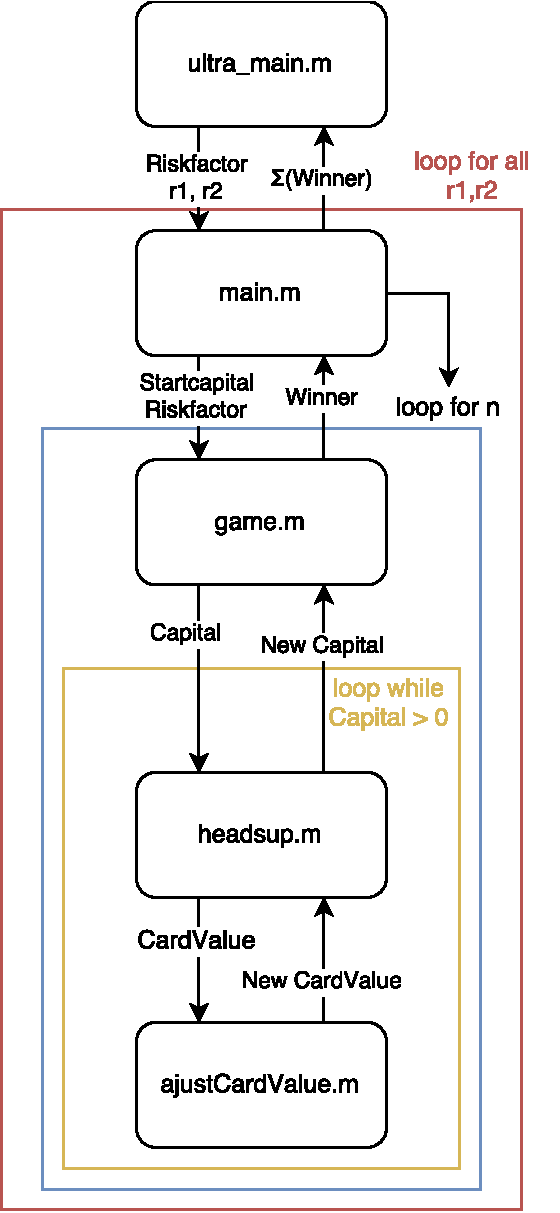
\includegraphics[width=\textwidth]{Graphics/diagram_senkrecht.pdf}
%\end{minipage}
%\begin{minipage}{0.48\textwidth}
%For better overview the script consists of a main file that repeatedly calls a function \textit{game.m}, which simulates a complete game. The function \textit{game.m} calls a function \textit{headsup.m} that simulates one hand, until one player has run out of money (game complete). The function \textit{game.m} is called by the function{main.m}, where all relevant variabes, relevant for the simulation are defined.
%After multiple tests an additional script \textit{ultramain.m} has been written to feed {main.m} with different risk-values.\\
%\end{minipage}
%
%
%
%%%%%
%
%
%%%%
%%%%%%
%%For better overview the script consists of a main file that repeatedly calls a function \textit{game.m}, which simulates a complete game. The function \textit{game.m} calls a function \textit{headsup.m} that simulates one hand, until one player has run out of money (game complete). The function \textit{game.m} is called by the function{main.m}, where all relevant variabes, relevant for the simulation are defined.
%%After multiple tests an additional script \textit{ultramain.m} has been written to feed {main.m} with different risk-values.\\
%%
%%\begin{figure}[h!]
%%\centering
%%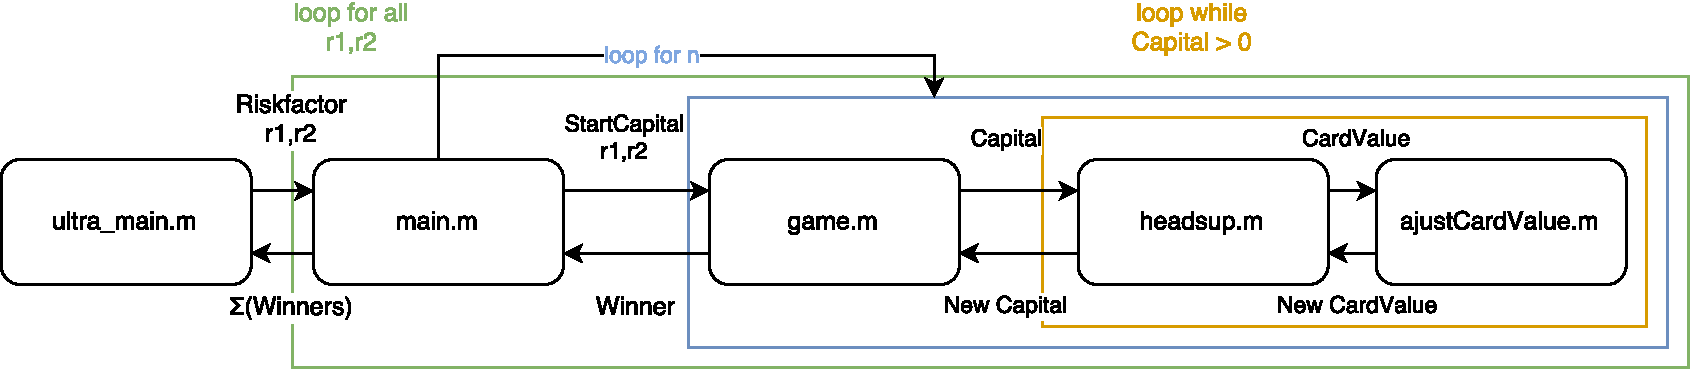
\includegraphics[scale=0.55]{Graphics/diagramm_waagrecht.pdf}
%%\caption{Simplified sceme of relations of relevant scriptes\label{Abbildung}}
%%\end{figure}
%
%
%
%\subsubsection{adjustCardValue.m}
%At the heart of this simulation lies the adjustCardValue function, which recalculates the card value of a player. Important criteria are that the cards correlate with each other, so if a player has good cards it is likely that his hand is still good when a new phase is played, but also should it be possible to for a value to reach the whole spectrum of card quality from 0 to 1. This is important because for an example in real Texas Holdem if one has a bad starting hand but with some luck to have the best hand possible after the flop. Hence every value should be possible but not with the same probability.\\
%The way we implemented this mechanism is that the function receives the old card value and a number between 0 and 1 we call sigma. Then the function calculates the new value based on the normal distribution where the old card value sets the middle of the curve and the sigma determines how fast probability fades down to zero. A very high sigma means that the recalculated value has the chance to be on the whole spectrum and a very low sigma computes a new card value close to the old one.
%We chose the sigma for the flop as 0.4 because there three new cards are dealt and a big variety of outcomes is needed. In the next two rounds where only one card is dealt the current card value has to be stable so the chosen sigma there is 0.2.\\
%The first line of Table ??? shows the card value that needs to be recalculated and line two represents the average of a hundred new card values. This shows that with a sigma of 0.2 the average is pretty stable. The values at the top and bottom differ a little bit more because there is a set boundary at zero and one. Hence at 0.9 there are maybe as many values above this number as there are below but the ones underneath reach much lower.\\
%Table two shows the highest and lowest possible resulting value of certain incoming number over a hundred played games. Whereas the first line represents the old card value, line two the highest and line three the lowest possible value. This data supports the choice of a sigma of 0.4 because every value has the potential to reach the whole spectrum.
%
%\begin{table}[]
%\centering
%\caption{Old and new card values with a sigma 0.2}
%\label{my-label}
%\begin{tabular}{lllllllll}
%0.1 & 0.2 & 0.3 & 0.4 & 0.5 & 0.6 & 0.7 & 0.8 & 0.9\\
%\addlinespace
%0.177 & 0.224 & 0.312 & 0.401 & 0.504 & 0.616 & 0.645 & 0.766 & 0.787 \\   
%\end{tabular}
%\caption{Highest and lowest possible card values with a sigma 0.4}
%\label{my-label}
%\begin{tabular}{lllllllll}
%0.1 & 0.2 & 0.3 & 0.4 & 0.5 & 0.6 & 0.7 & 0.8 & 0.9\\
%\addlinespace
%0.9014& 0.9871 & 0.9972 & 0.9596 & 0.9984 & 0.9918 & 0.9992 & 0.9960 & 0.9944\\
%\addlinespace
%0.0045 & 0.0008 & 0.0008 & 0.0108 & 0.0035 & 0.0068 & 0.0962 & 0.0218 & 0.0071 \\   
%\end{tabular}
%\end{table}
%
%\subsubsection{headsup.m}
%The core function, on which the simulation is built around. Is called headsup.m. It simulates one poker hand and consists of up to four rounds, where players can bet money on their win. At the end of a hand a showdown determines the winner, who can increase his capital by up to four betValues, while the losers capital decreases by the same amount.\\
%%sketchy \renewcommand{\arraystretch}{1.4}
%
%
%
%
%
%
%\begin{center}
%\begin{tabular}{c c}
%Inputs & Outputs\\
%
%\hline
%CapitalP1,-P2 & CapitalP1,-P2\\
%
%risk factorP1,-P2\\
%BetValue\\
%\end{tabular}\\
%\end{center}
%
%
%
%
%
%
%At the beginning of headsup each player gets a random (Card-)value Val between 0 and 1, this value replaces his two handcards in this simplified simulation. In a next step the player with a blind is forced to place this blind in the pot. The other player can decide if he wants to place an equal amount in the pot.  Of course, the placement of money in the pot reduces the capital of a player. After both players decided to play (preflop), their card-values Val are altered in the next step, that should resemble the Flop of a normal poker game. Afterwards the players get another chance to place a bet, which is followed by the river, where once more both (Card-)values are slightly altered. This is followed by a last chance to place another bet before the showdown. In which the player with the better Card-Value wins the money in the pot.
%
%\subsubsection{game.m}
%The function game.m is used to call the function headsup. Like in real poker game.m continues to call headsup, until one player has run out of money. To do so a while loop has been used. Game.m has the following input variables:
%risk factorP1,-P2
%CapitalP1,-P2
%BetValue
%The output of the function game is the winning player.
%\subsubsection{main.m}
%In the function main.m all important variables are defined and passed on the function game.
%Additionally to that the variables needed to in the function main the number of games played is defined.
%Ultra-main: Is an additional script used to efficiently vary risk-factor one and two and to display the results in the form of a matrix.
%%%%%--------------List of Variables----------------%%%%
%
%
%%%%%--------------/List of Variables----------------%%%%
%
%
%
%

\section{Simulation Results and Discussion}

\subsection{Results of generic model}

\begin{figure}
\begin{center}
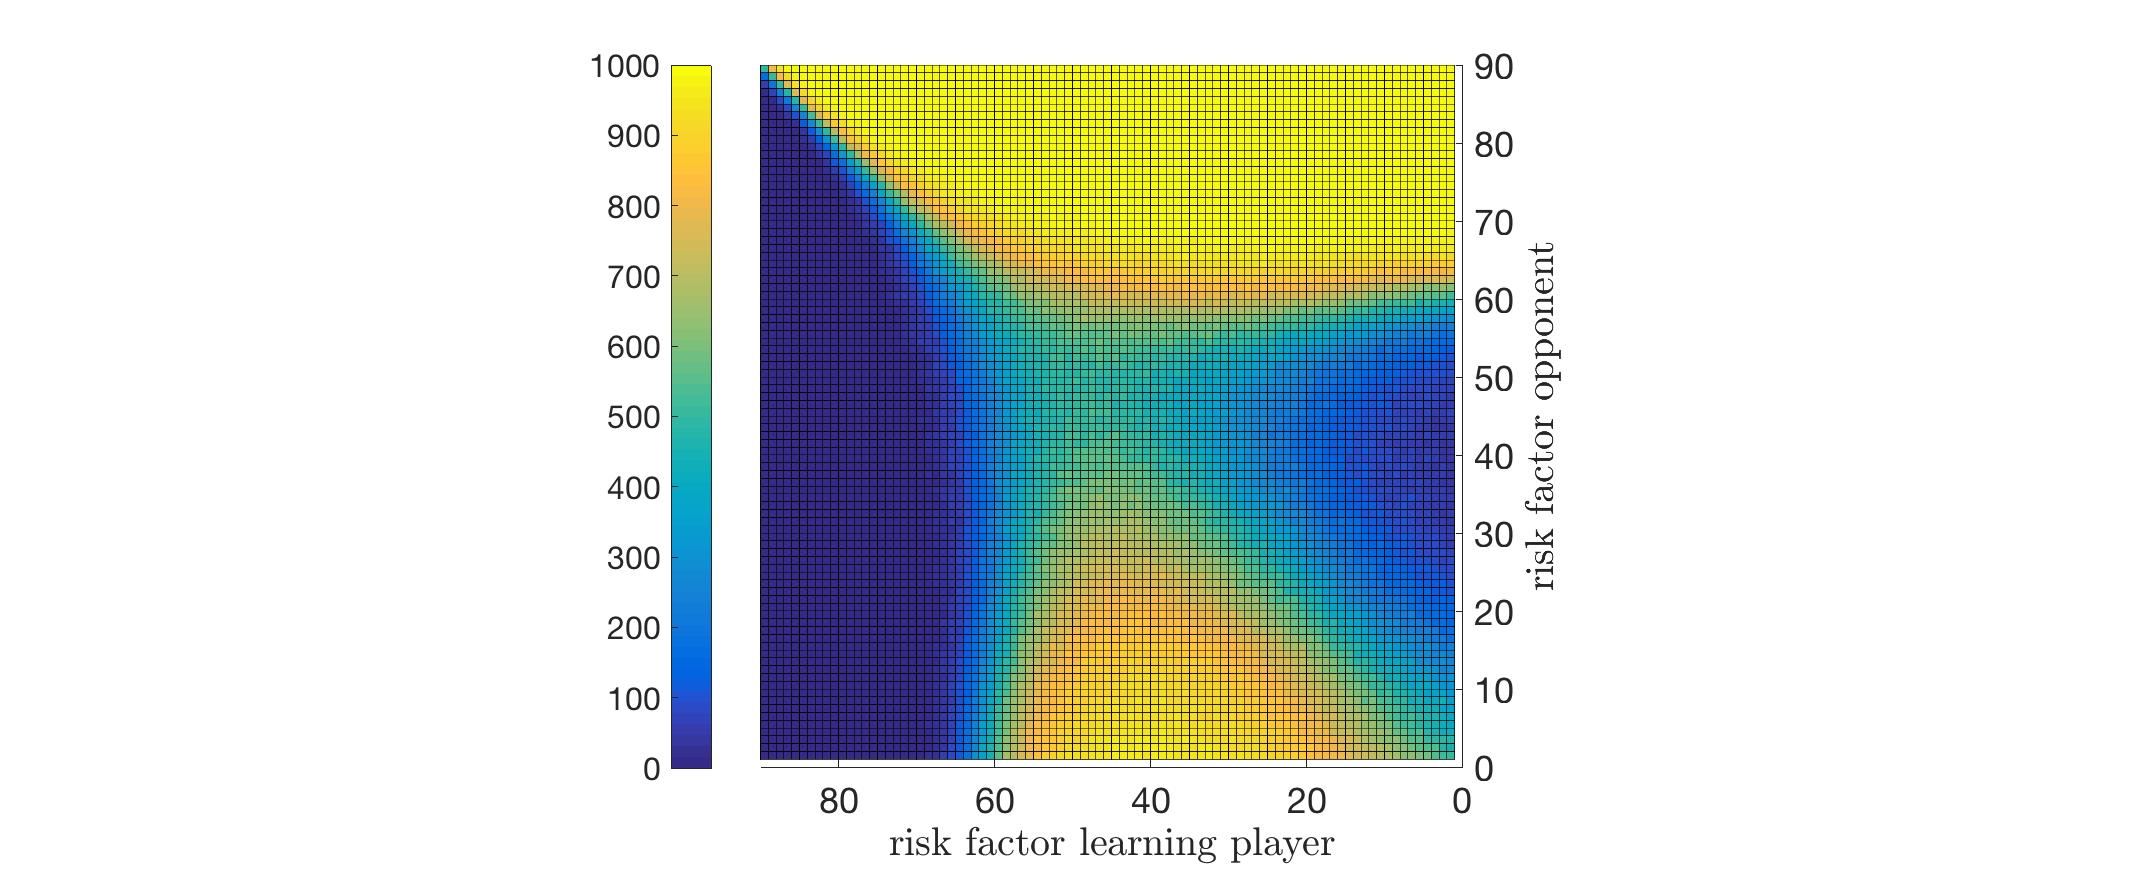
\includegraphics[scale=0.2]{Graphics/allDataPlot_BlindOn_1000Games_001Step_TopFlat.jpg}
\caption{Games won by player1 out of 1000\label{Topview of all Data}}
\end{center}
\end{figure}

\subsubsection{Generic model -- Results }
Figure \ref{Topview of all Data} shows how many games player1 has won out of a total of 1000, when both players started out with an equal amount of chips (50) and a fixed blind equal to the betValue of 1. The colour of every cell ($x=r, y=r2$) shows the number of games won by player1 with his risk factor $r1$ against player2 with a risk factor $r2$.\\
% 

On the diagonal ($r1=r2$) a green line can be seen, which shows that player1 and player2 have each won approximately half of all games played. Around this line the games won by a player are approximately antisymmetrically distributed, which means that both players did equally well when using the same risk factor.\\

%
A very passive strategy ($r > 0.63$) could not win any games, except against a more passive player. In this case, the less passive strategy occurred to be superior.\\
%

An aggressive strategy ($r < 0.5$) performed better. It could win against the very passive strategy (r opponent $> 0.63$). However, it clearly lost against all less aggressive strategies under 0.63 ($r < r$ opponent $< 0.63$).\\

Thus, there are two different patterns visible in Figure \ref{Topview of all Data}. One pattern ($r <0.5$), where the more passive player wins. And a second pattern ($r>0.63$), where the more active player wins.\\

Between these two patterns lies a transition area, where both risk factors are between 0.5 and 0.63. In this area the games were very balanced and not even an optimal counter-strategy did win more than 60\% of all games.\\

In the transistion area the change from where it is favorable to play passiv on to playing active occurs.

 \subsubsection{Generic model -- Interpretation}

The bad performance of the very passive strategy can be explained with two independent mechanisms. One being the blind that punishes the more passive player. The other being the card score dropping below the risk factor before the showdown, leading to a loss of all chips bet during that hand.\\
The aggressive player plays more games with weak hands, which means that he will lose more often in the case of a showdown.\\
Inside the area, where the game is balanced, all mentioned effects compensate each other.\\

The model weights the effect of a passive player dropping out after already having invested chips to heavily. In a real game of poker a player stays in the game, due to a comparison between his own odds and the pot. This effect is called pot odds.\\
Otherwise the simulation shows that the aggressive strategy (loose play) is favorable against an extreme passive strategy (tight play). This reflects the reality where blinds give the passive player a disadvantage in a heads up.\\

\subsection{Results of learning algorithms}

\begin{center}
\begin{figure}

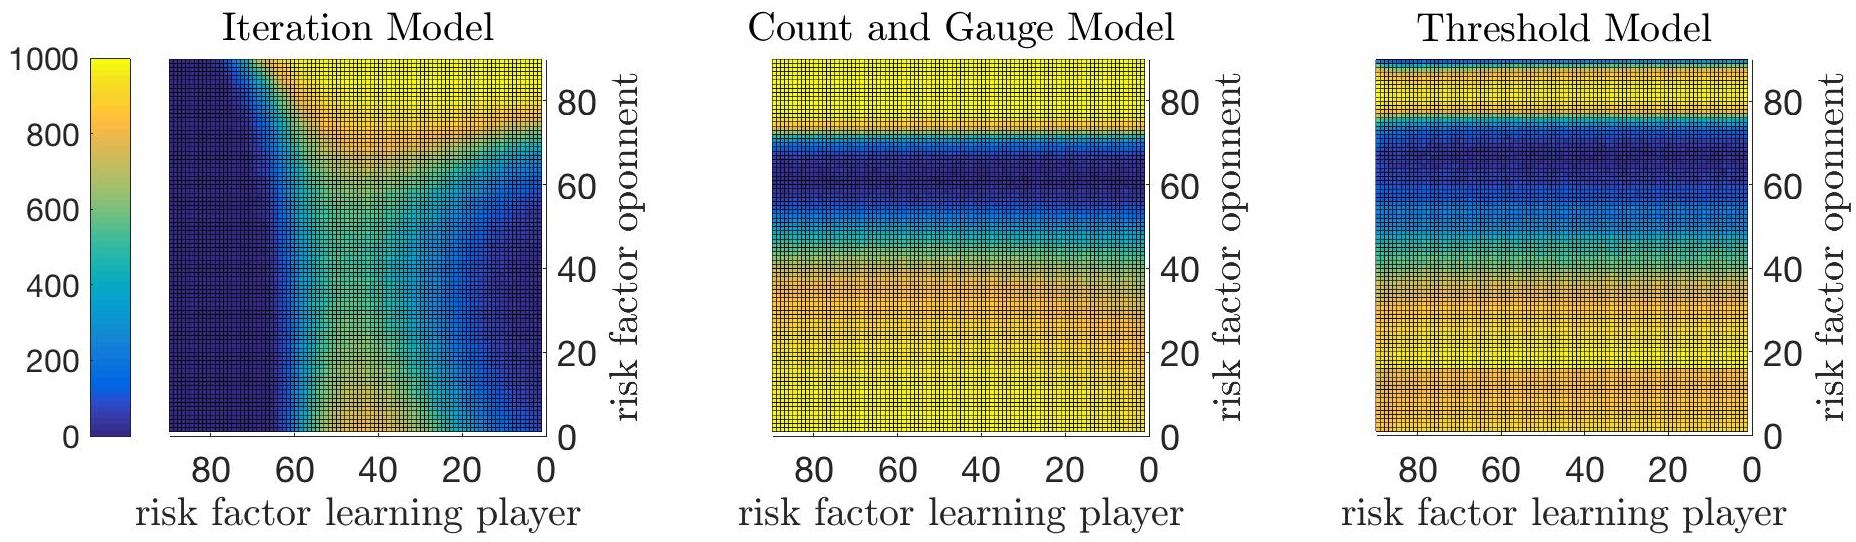
\includegraphics[scale=.23]{Graphics/OvViewLatex18}
\caption{Resulting win matrices for all three learning models. From left to right: threshold, count and gauge, iteration}
\label{LearningModelsAllDataOverview}

\end{figure}
\end{center}


\subsubsection{Iteration model}

The algorithm needs around 800 hands in order to leed to a good estimation for the optimal parameter r. This leads to good results for start capitals above 70 and to very good results at start capitals above 300 even with a very unfavorable starting strategy like r(0)=0.1.
\\

\begin{tabular}{ p{7.2cm}  p{7.2cm}}
\textbf{Advantages} & \textbf{Disadvantages}\\
The model has a great potential for different kinds of optimisation:
\begin{itemize}
\item Parameters used in the model can still be optimised in order to perform quicker
\item More cases for different scenarios could be made (different action for loss of one and loss of two)
\item The cards that the player could have taken into account in order to avoid a change in policy if he only had bad luck
\end{itemize}
& The algorithm is based on a simplified scenario, where the only reason for a loss is based on the strategy and never on luck. This leads in some cases to a change of policy even when it is not desired. This can be observed in the high standard deviation, even after having found a well estimated $r$. This behavior leeds to the algorithm loosing against extremely strong strategies due to its continous slight deviations from the optimum risk factor.\\ 
\end{tabular}

\subsubsection{Count and Gauge model}
The algorithm leads to a significant increase in the number of games won. Unfortunately in the region between 0.5 and 0.7 it was rather contra productive. In this region an adjustment of the otherwise solid algorithm is needed.
We relate this event to the transition from the “passive area” to the “active area”. The impact of luck can easily shift the estimation of ones opponent's risk factor into the wrong area which ultimately ends by choosing the wrong counterstrategy.\\


\begin{minipage}[t]{0.48\textwidth}
\textbf{Advantages}\\
%\addlinespace
With an increasing number of rounds the estimation continuously becomes better\\
On a long run he will always play the most suitable strategy and optimise his return\\
It reaches a good estimation of the opponent's risk factor already after a few rounds\\
The algorithm could also use the rounds where the other player has to pay the blind by counting the number of consecutive rounds he plays and applies the same strategy just by including the models standard deviation into the calculation. This would lead to a faster estimation of the opponent's risk factor
\end{minipage}\hfill
\begin{minipage}[t]{0.48\textwidth}
\textbf{Disadvantages}\\
%\addlinespace
The algorithm requires a precise knowledge of all possible outcomes and therefore is only applicable in the same circumstances the data was obtained\\
\end{minipage}

\subsubsection{Threshold model}

Figure \ref{LearningModelsAllDataOverview} shows that the resulting wins are independent from the learning player's risk factor because results are nearly constant along a horizontal line. It is visible that the algorithm does not have the same effectiveness for all opponent-strategies. For an opponent risk factor $r \in [0,0.4]$  and also around 0.8 the algorithm is really succesfull, as can be seen with the highly yellow areas in the plot, which represent a lot of wins for the learning player. From the green band at an opponents risk factor of around 0.45 it can be seen that wins are equally balanced around this point. In the blue area for an opponents risk factor between 0.5 and 0.75 wins for the learning player are infrequent. This mean that there the algorithm fails to provide an advantage over the opponent.\\

\begin{figure}
\begin{center}
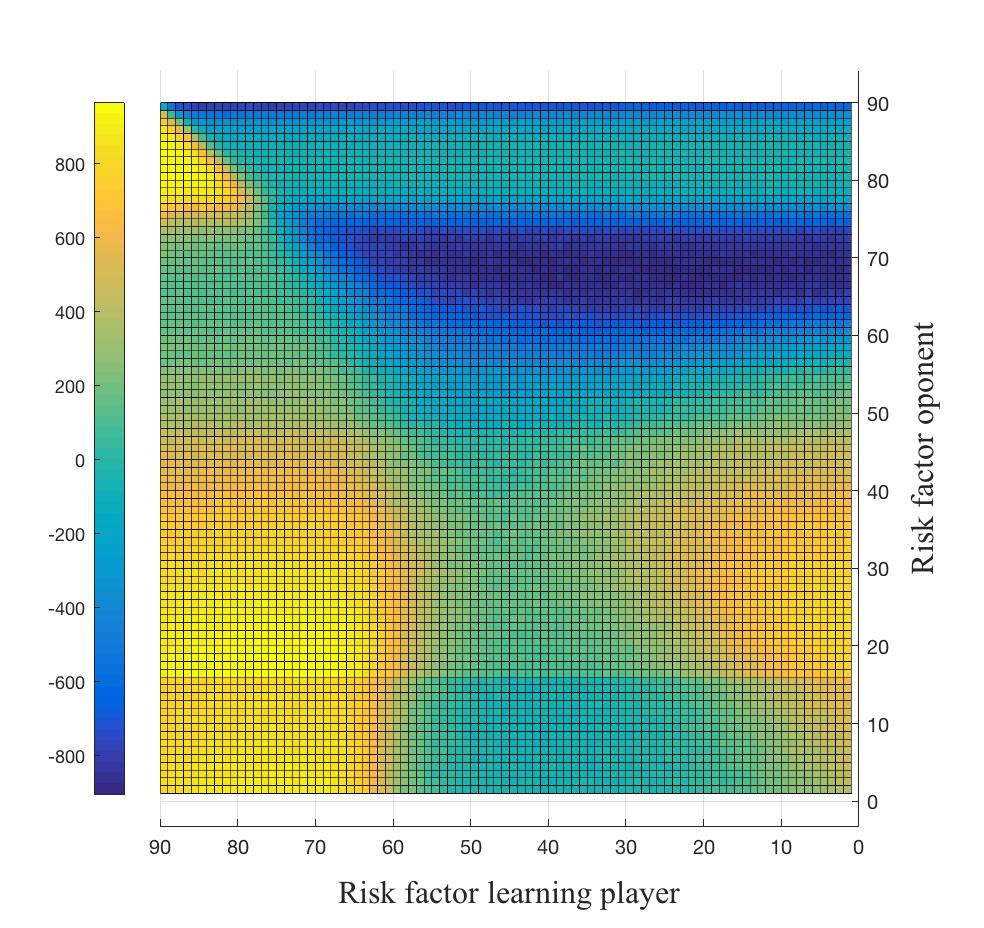
\includegraphics[scale=.3]{Graphics/allDataWins_Threshold_Difference}
\end{center}
\caption{Topview of difference from results of threshold learning model and generic model with blinds}
\label{allDataWins_Threshold_Difference}
\end{figure}

By subtracting the resultant matrix from generic model with blinds from that of the learning algorithm it can be visualized where the threshold learning algorithm improves the game results and where it fails to do so. This is shown in figure \ref{allDataWins_Threshold_Difference}. The highly yellow areas show a drastic improvement in performance, whereas the green areas represent scopes where the performance could only be slightly changed or even remained the same. The deep blue areas show scopes in which the learning players performance has declined drasticly.\\

The behaviour of the learning model in the green and yellow areas can be explained as follows: since the performance from the learning player in the green areas was already good, with the generic model no big improvement could be realised. The difference in wins therefore leveled off in these sections. The yellow areas underly low performance regions in the generic model with blinds, thus a big improvement can be realised and the difference in wins rocketed.\\

What remains to explain are the not expected blue areas. In the blue area at a risk factor of 0.9 the opponent plays extremely passive. Hence a showdown seldomly occurs and the learning algorithm cannot take effect. However this can only explain the failure of the learning aspect of the algorithm but not the loss of the learning player. The other blue area's behaviour can be explained by the addition of two effects. Firstly the gradient of the generic result matrix is extremly steep, thus already a slight misestimate in the opponent's risk factor can lead to a big change in the optimal risk factor for the learning player. Secondly because in the turn the opponent can also play a hand up to 0.15 lower than his risk factor the estimation for his risk factor can also be shifted downwards by up to 0.15 and therefore lead to a miscalculation in the optimal risk factor for the learning player.


\subsection{Comparison of learning algorithm performances}


\begin{table}[]
\centering
\caption{Learning models overview figures}


\label{Learning models overview}
\begin{tabular}{lcccccc}
\cline{2-7}
                                           & \multicolumn{2}{c}{\# Games won}                      & \multicolumn{2}{c}{\# Hands played}                   & \multicolumn{2}{c}{$\Delta$games won} \\ \cline{2-7} 
\multicolumn{1}{c|}{}                       & \multicolumn{1}{c|}{$\mu$} & \multicolumn{1}{c|}{$\sigma$} & \multicolumn{1}{c|}{$\mu$} & \multicolumn{1}{c|}{$\sigma$} & \multicolumn{1}{c|}{$\mu$} & $\sigma$ \\ \hline


\multicolumn{1}{l|}{Iteration model}           & 647.55                     & \multicolumn{1}{c|}{335.5068}         & 110020                     & \multicolumn{1}{c|}{748600}   & 147.7569                            & 198.3177        \\ \hline
\multicolumn{1}{l|}{Count and gauge model} & 690.6369                   & \multicolumn{1}{c|}{343.1811} & 709.3543                   & \multicolumn{1}{c|}{342.5163} & 190.8446                   & 477.6301 \\ \hline
\multicolumn{1}{l|}{Threshold model}       & 605.7777                   & \multicolumn{1}{c|}{301.3260} & 1565                       & \multicolumn{1}{c|}{1854}     & 105.9853                   & 501.7773 \\ \hline


\end{tabular}
\end{table}


In table \ref{Learning models overview} some characteristic values for the learning algorithms are displayed. Therefore the mean and the standard deviation of the resulting-wins-matrix, total-hands-played-matrix and the difference-in-wins-matrix with and without the learning algorithm have been calculated. By comparing the mean of games won it can be seen, that the count and gauge model is the most successful algorithm in terms of most wins created. Yet due to the high standard deviation in games won, also the most inconsistent. From the standard deviation of difference in games won it can be distinguished that the iteration model is the most balanced overall, leading to small improvements for all different opponent strategies. In comparison thereto the threshold- and count and gauge model are not successful against every opponent, but if they are, they create a high yield. \\

Lastly the time efficiency has to be considered: Clearly the count and gauge algorithm is the one leading to a victory the quickest, as its low mean in hands played shows. On the other hand the iteration is the most time consuming. While being the most effective for every opponent its enormous mean amount of hands played leaves it to be essentially useless in practice.


\section{Robustness of results and influence of sigma}

To draw some conclusions from our model we had to ensure that our model is robust enough. We performed thousand games a thousand times and found a standard deviation of 7.7 for the wins.\\

To the function adjustCardValue.m a sigma for the flop is needed that leads to a big variety of outcomes because three new cards are dealt in that round. Still the difference in the card value before and after new cards cannot be too wide, otherwise all correlation is lost. In the next two rounds, the turn and the river, where only one card is dealt the current card value has to be somewhat stable.\\

We chose the combination of 0.4/0.2/0.2 to be the one that represents a game of Texas Hold'em the best. \\

We ran some simulations with different sigmas and saw that for each combination the resulting graph has the same shape but is shifted to the left or the right of the x and y scale.

Sigma have been tested on their reach from 0 to 1 and lowest/highest possible value for each risk factor. The results can be found on GitHub\footnote{https://github.com/atlas000/project-poker-msssm}.



\section{Summary and Outlook}
\subsection{Summary}
The most important understanding we gained from our simulation was definitely that there is a transition between when it is favourable to play aggressively and when to play rather passively. This can be translated into the applicable technique that if your opponent plays less than every third hand, one will win more, if one plays more aggressively. On the other side of this barrier, if the opponent plays more than every second hand, playing a bit more conservatively will increase winnings in the long term. This rule can easily be implemented by just counting the number of times the opponent pays the blind when he is not forced to, divided by the amount of times it was not the case.\\

Our learning algorithm overall increased the performance, but all encountered big problems in the transition region. This reflects the complexity of poker even under simplified conditions and that there is no magical formula even when the opponent plays extremely balanced.\\

Nevertheless we learned from our approach that by keeping track of the opponent's decisions, there can be a lot of insights gained about his strategy. After a few rounds played then the easy rule mentioned above can be applied to gain an advantage. In case the estimated risk factor of the opponent lies within the transition area, the result has to be treated with caution, as the stubborn execution can lead to the opposite the desired results as proved by the count and gauge algorithm.\\

\subsection{Outlook and Limitations}
This project is developable in many kind of ways. We had thought of some different parameters one could implement. \\
One of them was a blind that would increase over time. This is how it is played in real Texas Holdem with the motive to punish passive play. Because of that it would have been interesting to observe what difference it would have made in our simulation, also since our games lasted up to over a thousand hands and this is far away from reality.\\

One could also have tweaked the capital/betValue ratio in general. Possible outcomes could have been that with a certain ratio the aggressive player gets punished because his loosing hands include bigger pots or the conservative player looses more often because games are more fast paced.\\

Another extremely interesting feature could have been giving the players the option to decide with how much they wanted to raise the pot. Currently, one chip is the only option but how would the outcome of a game be if they could bet a larger and varying amount. If that was the case, card evaluation needed to be different. A player then not only has to take his own cards in to the decision to play or drop out but also how much money his opponent has bet in this round. Furthermore, would this change have opened the opportunity for a player to bluff his counterpart, this means pretending to have better cards than what he actually has. Now the more active player might get rewarded for his play style.\\

The possibility of checking could also have been included. Checking is doing nothing when your opponent has not bet any chips. This variation would need a distinct playing order and that would put the  one, who has to show his cards first in a showdown, into a disadvantage. All these factors could play a role in developing a winning algorithm.\\

Other variations that certainly would lead to different discoveries but would make the program much more complex are coding ''real'' cards with their actual probabilities to show up in a hand but also including more than two players which might would change the power dynamics between active and passive players.


\section{References}

\section{Appendix}
\subsection{Source Code}
\subsection{Variable documentation}
\subsubsection{Variables from generic model}




\begin{itemize}

\item	\textbf{Scripts:} \textcolor{red}{ultra\_main(um), main(m), game(g), headsUp/headsUp2(h), adjustCardValue(acv)} \\

\item	\textbf{playerP1, playerP2, \textcolor{red}{general}:} Vector with 4 entries representing all important variables from one player.
\begin{enumerate}
	\item risk factor for player
	\item capital from player
	\item card value from player, is a random number between 0 and 1
	\item total bet from player
	\item free variable for learning implementation
\end{enumerate}		
	
	
	
	
\item	\textbf{allData \textcolor{red}{um}:}  Matrix containing number of Wins from player 1 one for varying risk factors\\
	
\item	\textbf{r1, r2 \textcolor{red}{um}:}  iteration variables representing risk factors for players 1 and 2\\

\item	\textbf{betValue \textcolor{red}{m,h}:} represents the amount a player can bet on his win or the amount by which the pot can be increased per round per person \\

\item	\textbf{n \textcolor{red}{m}:}  iteration variable for determining how many games are being simulated, hence determining the accuracy of the monte carlo approach\\

\item	\textbf{riskfactorP1, riskFactorP2 \textcolor{red}{m}:}  variables representing the risk factors for both players\\

\item	\textbf{startCapital \textcolor{red}{m}:} determines the capital at the beginning of the game for both players. \\

\item	\textbf{winsP1 \textcolor{red}{m}:} amount of total wins by player 1, used as output to the function main.m  \\

\item	\textbf{winner \textcolor{red}{m,g}:} stores the the winner of the game simulated: if 0 winner is player 2, if 1 winner is player 1, used as output to the function game.m\\

\item	\textbf{counter \textcolor{red}{g}:} counts amount of hands played in one game \\

\item	\textbf{decide\_who\_starts \textcolor{red}{g}:} used to determine whose turn it is to start with betting, if 0 player 2 begins, if 1 player 1 begins  \\

\item	\textbf{pot \textcolor{red}{h}:}  stores the total amount of money betted by both players\\

\item	\textbf{capP1, capP2 \textcolor{red}{}:} output variables to headsUp.m function storing the capital of the corresponding player after having played the hand\\

\item	\textbf{newRandValue \textcolor{red}{acv}:} output to adjustCardValue.m function, stores the newly generated cardvalue  \\

\item	\textbf{sigma \textcolor{red}{acv}:} theoretically the standard deviation of a normally distributed random value, here used to determine the range of adjustement for the function adjustCardValue.m \\

\end{itemize}

\subsubsection{Variables from learning models}
\paragraph{Threshold model}
\begin{itemize}
\item	\textbf{Scripts:} \textcolor{red}{ultra\_main(um), main(m), game(g), headsUp/headsUp2(h), adjustCardValue(acv), adjustRiskFactor(arf)} \\

\item	\textbf{totalCounter \textcolor{red}{m}:} used to store total amount of hands played per game  \\

\item	\textbf{playerP1(5) \textcolor{red}{g}:} stores the risk factor of player 2 as it is currently estimated by player 1  \\

\item	\textbf{startRiskFactor \textcolor{red}{h}:} input to headsup.m function, stores the risk factor from player 2 as estimated by player 1 before the respective hand  \\

\item	\textbf{estRiskFactor \textcolor{red}{h}:} output from headsup.m function, stores the risk factor from player 2 as estimated by player 1 after the respective hand   \\

\item	\textbf{newRiskFactor \textcolor{red}{arf}:}  output from adjustRiskFactor.m function, stores newly generated risk factor\\

\item	\textbf{opponentRiskFactor \textcolor{red}{arf}:} input to function adjustRiskFactor.m, currently estimated risk factor from opponent player \\

\item	\textbf{refSurf \textcolor{red}{arf}:} two-variable function which represents amount of wins for player 1 in dependence of the respective risk factors \\

\item	\textbf{funVector \textcolor{red}{arf}:} parameterisation of refSurf at point of opponentRiskFactor \\

\end{itemize}






\end{document}  



 
